\chapter{Governing equations and the vertical coordinate}\label{ch:eq}

The ARW core solves the fully compressible, non-hydrostatic Euler equations for a moist atmosphere, written in flux
form on a mass-based vertical coordinate \citep{skamarock2019}. This chapter states the equations as the code solves
them, defines the hybrid coordinate exactly as \code{real.exe} and \code{wrf.exe} compute it, and connects every term
to the routine that evaluates it. The numerical methods follow in \cref{ch:time,ch:adv}.

\section{The hybrid mass coordinate}

WRF's vertical coordinate $\eta$ is defined through the \emph{dry hydrostatic pressure} $p_d$. It runs from
$\eta = 1$ at the surface to $\eta = 0$ at the model top, where the pressure is the constant $p_t$. With
\code{hybrid_opt = 2}, the coordinate is terrain-following near the ground and becomes a pure pressure coordinate
aloft:
\begin{equation}
  p_d(x, y, \eta, t) = B(\eta)\,\bigl(p_s(x,y,t) - p_t\bigr) + \bigl(\eta - B(\eta)\bigr)\,(p_0 - p_t) + p_t ,
  \label{eq:hybrid}
\end{equation}
where $p_s$ is the dry surface pressure and $p_0 = 1000$~hPa. The function $B$ goes from 1 at the surface to 0 at
and above the level $\eta_c$ (\code{etac}, 0.2 by default). WRF uses the polynomial of
\src{dyn_em/nest_init_utils.F}{compute_vcoord_1d_coeffs}:
\begin{equation}
  B(\eta) = \frac{b_1 + b_2\eta + b_3\eta^2 + b_4\eta^3}{(1-\eta_c)^4}
  \quad (\eta \ge \eta_c), \qquad B(\eta) = 0 \quad (\eta < \eta_c),
  \label{eq:B}
\end{equation}
with
\begin{align*}
  b_1 &= 2\eta_c^2(1-\eta_c), & b_2 &= -\eta_c\,(4 - 3\eta_c - \eta_c^3), \\
  b_3 &= 2\,(1-\eta_c^3), & b_4 &= -(1-\eta_c^2),
\end{align*}
and $B = 1$ exactly at the lowest full level. With \code{hybrid_opt = 0}, $B(\eta) = \eta$, the classic
terrain-following coordinate.

\begin{figure}[ht]
\centering
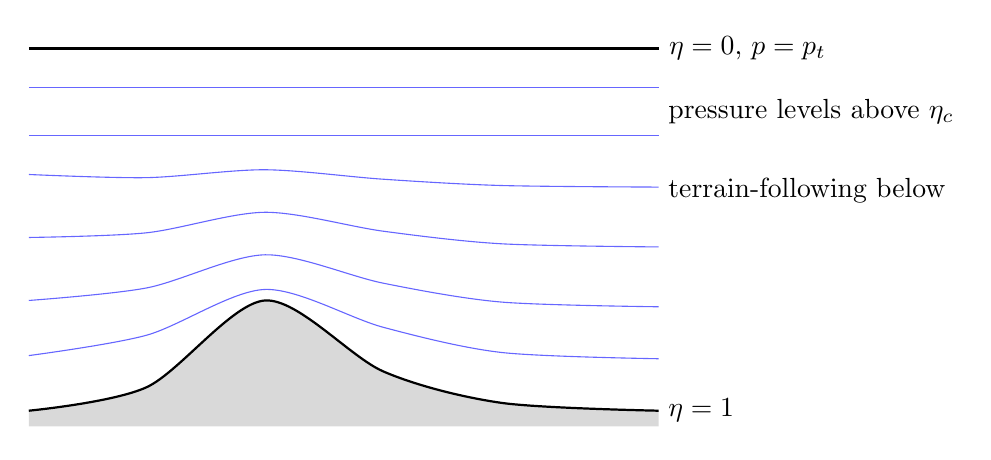
\begin{tikzpicture}[x=1cm,y=1cm]
  \fill[black!15] (0,0) -- plot[smooth] coordinates {(0,0.2) (1.5,0.5) (3,1.6) (4.5,0.7) (6,0.3) (8,0.2)} -- (8,0) -- cycle;
  \draw[thick] plot[smooth] coordinates {(0,0.2) (1.5,0.5) (3,1.6) (4.5,0.7) (6,0.3) (8,0.2)};
  \foreach \f/\h in {0.8/0.7, 0.6/1.4, 0.4/2.2, 0.2/3.0} {
    \draw[blue!60] plot[smooth] coordinates {(0,0.2+\h) (1.5,0.5*\f+\h+0.06) (3,1.6*\f+\h-0.3*\f) (4.5,0.7*\f+\h) (6,0.3*\f+\h) (8,0.2*\f+\h)};
  }
  \foreach \h in {3.7, 4.3} { \draw[blue!60] (0,\h) -- (8,\h); }
  \draw[thick] (0,4.8) -- (8,4.8) node[right] {$\eta = 0$, $p = p_t$};
  \node[right] at (8,0.2) {$\eta = 1$};
  \node[right] at (8,3.0) {terrain-following below};
  \node[right] at (8,4.0) {pressure levels above $\eta_c$};
\end{tikzpicture}
\caption{Coordinate surfaces of the hybrid coordinate (schematic). Near the ground they follow the terrain; their
undulation decays with height and vanishes above $\eta_c$, where they are surfaces of constant pressure.}
\label{fig:hybrid}
\end{figure}

The code stores \cref{eq:hybrid} as four one-dimensional coefficient arrays, on full levels (suffix \code{f}) and
half levels (suffix \code{h}). With $\mu = p_s - p_t$, the dry column mass:
\begin{align}
  c_3 &= B(\eta), & c_4 &= (\eta - B)(p_0 - p_t), & p_d &= c_3\,\mu + c_4 + p_t, \label{eq:c34}\\
  c_1 &= \frac{\mathrm{d}B}{\mathrm{d}\eta}, & c_2 &= (1 - c_1)(p_0 - p_t), &
  \mu_d &\equiv \pd{p_d}{\eta} = c_1\,\mu + c_2 . \label{eq:c12}
\end{align}
Here $\mu_d$ is the \emph{metric} of the coordinate: the dry-air mass per unit area per unit $\eta$. Wherever the
equations below contain $\mu_d$ at a level, the code writes \code{(c1(k)*mut(i,j)+c2(k))}, with \code{mut} the column
mass $\mu$ of the point and \code{c1}, \code{c2} the coefficients of that level. With \code{hybrid_opt = 0},
$c_1 = 1$ and $c_2 = 0$, so $\mu_d = \mu$ at every level.

\section{Prognostic variables}

The equations are written for mass-coupled (flux) variables. With the map-scale factors $m_x$, $m_y$ of the
projection (\cref{ch:system,ch:cor}):
\begin{equation}
  U = \frac{\mu_d u}{m_y},\quad V = \frac{\mu_d v}{m_x},\quad W = \frac{\mu_d w}{m_y},\quad
  \Omega = \frac{\mu_d \dot\eta}{m_y},\quad \Theta_m = \mu_d\,\theta_m,\quad Q_m = \mu_d\,q_m .
\end{equation}
\begin{itemize}
  \item $u, v, w$ are the velocity components; $\dot\eta = \mathrm{d}\eta/\mathrm{d}t$ is the coordinate velocity.
  \item $\theta_m = \theta\,(1 + (R_v/R_d)\,q_v)$ is the moist potential temperature (\code{use_theta_m = 1}).
  \item $q_m$ are the mixing ratios of water vapor, cloud water, rain, ice, snow and graupel, and other scalars.
  \item $\phi = gz$ is the geopotential.
\end{itemize}
The inverse density of dry air is $\alpha_d = 1/\rho_d$. The full inverse density is
$\alpha = \alpha_d\,(1 + q_v + q_c + q_r + q_i + q_s + q_g)^{-1}$.

In the code, the domain type \code{grid} holds (\cref{ch:arch}):
\begin{center}
\begin{tabular}{ll}
\toprule
Field & Meaning \\
\midrule
\code{u_2}, \code{v_2}, \code{w_2} & $u$, $v$, $w$ \\
\code{ru}, \code{rv}, \code{rw}, \code{ww} & the coupled $U$, $V$, $W$, $\Omega$ \\
\code{mu_2}, \code{mub} & $\mu'$ and $\bar\mu$; \code{mut} $= \bar\mu + \mu'$ \\
\code{t_2} & $\theta_m - T_0$ with $T_0 = 300$~K \\
\code{ph_2}, \code{phb} & $\phi'$ and $\bar\phi$ \\
\code{p}, \code{pb} & $p'$ and $\bar p$ \\
\code{al}, \code{alb}, \code{alt} & $\alpha'_d$, $\bar\alpha_d$, $\alpha_d$ \\
\code{moist(:,:,:,n)} & $q_m$, one slot per species \\
\bottomrule
\end{tabular}
\end{center}

\section{The equations in flux form}

With the map factors and moisture, the ARW equations are \citep{skamarock2019}:
\begin{align}
  \partial_t U + m_x\bigl[\partial_x(Uu) + \partial_y(Vu)\bigr] + \partial_\eta(\Omega u)
    + \frac{m_x}{m_y}\frac{\alpha}{\alpha_d}\Bigl[\mu_d\,(\partial_x\phi + \alpha_d\,\partial_x p)
    + \partial_\eta p\;\partial_x\phi\Bigr] &= F_U , \label{eq:U}\\
  \partial_t V + m_y\bigl[\partial_x(Uv) + \partial_y(Vv)\bigr] + \frac{m_y}{m_x}\partial_\eta(\Omega v)
    + \frac{m_y}{m_x}\frac{\alpha}{\alpha_d}\Bigl[\mu_d\,(\partial_y\phi + \alpha_d\,\partial_y p)
    + \partial_\eta p\;\partial_y\phi\Bigr] &= F_V , \label{eq:V}\\
  \partial_t W + \frac{m_x m_y}{m_y}\bigl[\partial_x(Uw) + \partial_y(Vw)\bigr] + \partial_\eta(\Omega w)
    - \frac{g}{m_y}\Bigl[\frac{\alpha}{\alpha_d}\,\partial_\eta p - \mu_d\Bigr] &= F_W , \label{eq:W}\\
  \partial_t \Theta_m + m_x m_y\bigl[\partial_x(U\theta_m) + \partial_y(V\theta_m)\bigr]
    + m_y\,\partial_\eta(\Omega\theta_m) &= F_{\Theta_m} , \label{eq:T}\\
  \partial_t \mu_d + m_x m_y\bigl[\partial_x U + \partial_y V\bigr] + m_y\,\partial_\eta\Omega &= 0 , \label{eq:mu}\\
  \partial_t \phi + \mu_d^{-1}\Bigl[m_x m_y\,(U\partial_x\phi + V\partial_y\phi) + m_y\,\Omega\,\partial_\eta\phi
    - m_y\, g\, W\Bigr] &= 0 , \label{eq:phi}\\
  \partial_t Q_m + m_x m_y\bigl[\partial_x(Uq_m) + \partial_y(Vq_m)\bigr] + m_y\,\partial_\eta(\Omega q_m)
    &= F_{Q_m} . \label{eq:Q}
\end{align}
The right-hand sides $F$ hold the Coriolis and curvature terms (\cref{ch:cor}), mixing and diffusion
(\cref{ch:turb}) and the physics tendencies (\cref{ch:phys}). The system is closed by two diagnostic relations:
the hydrostatic definition of the dry inverse density and the equation of state,
\begin{equation}
  \partial_\eta\phi = -\alpha_d\,\mu_d , \qquad
  p = p_0\left(\frac{R_d\,\theta_m}{p_0\,\alpha_d}\right)^{\gamma}, \quad \gamma = \frac{c_p}{c_v}.
  \label{eq:hydro-diag}
\end{equation}
The first relation does not make the model hydrostatic. Non-hydrostatic pressure departures enter through $p$, which
is computed from the equation of state, not from the column mass.

Integrating \cref{eq:mu} over the column, with $\Omega = 0$ at the surface and the top, gives the tendency of the
column mass and, by integrating partially, the coordinate velocity $\Omega$ on every level. This is how WRF diagnoses
the vertical mass flux: \src{dyn_em/module_big_step_utilities_em.F}{calc_ww_cp} on the large step and
\src{dyn_em/module_small_step_em.F}{advance_mu_t} on the acoustic step (\cref{ch:time}).

\section{Perturbation form}

The model integrates perturbations from the hydrostatically balanced base state of \cref{ch:icbc}:
$p = \bar p + p'$, $\phi = \bar\phi + \phi'$, $\alpha_d = \bar\alpha_d + \alpha'_d$,
$\mu_d = \bar\mu_d + \mu'_d$. Because the base state satisfies the hydrostatic relation exactly,
$\partial_\eta\bar p = -\bar\mu_d$ and $\partial_\eta\bar\phi = -\bar\alpha_d\bar\mu_d$, the pressure-gradient
terms become
\begin{align}
  \text{in } U:&\quad \frac{m_x}{m_y}\frac{\alpha}{\alpha_d}\Bigl[\mu_d\,(\partial_x\phi' + \alpha_d\,\partial_x p'
     + \alpha'_d\,\partial_x\bar p) + \partial_x\phi\,(\partial_\eta p' - \mu'_d)\Bigr], \label{eq:pgf-pert}\\
  \text{in } W:&\quad -\frac{g}{m_y}\frac{\alpha}{\alpha_d}\Bigl[\partial_\eta p'
     - \bar\mu_d\,(q_v + q_c + q_r + q_i + q_s + q_g)\Bigr] + \frac{g}{m_y}\,\mu'_d , \label{eq:buoy-pert}
\end{align}
and the hydrostatic relation for the perturbations is
\begin{equation}
  \partial_\eta\phi' = -\bigl(\bar\mu_d\,\alpha'_d + \alpha_d\,\mu'_d\bigr).
  \label{eq:hydro-pert}
\end{equation}
In the code:
\begin{itemize}
  \item \cref{eq:pgf-pert} is evaluated by \src{dyn_em/module_big_step_utilities_em.F}{horizontal_pressure_gradient}
    on the large step and by \src{dyn_em/module_small_step_em.F}{advance_uv} on the acoustic step;
  \item \cref{eq:buoy-pert} is split between \src{dyn_em/module_big_step_utilities_em.F}{pg_buoy_w} (large step)
    and the implicit solve in \src{dyn_em/module_small_step_em.F}{advance_w};
  \item the factor $\alpha/\alpha_d = (1 + q_{\mathrm{tot}})^{-1}$, averaged to the $u$, $v$ and $w$ points, is
    computed once per stage by \src{dyn_em/module_big_step_utilities_em.F}{calc_cq} (\code{cqu}, \code{cqv},
    \code{cqw}).
\end{itemize}

\section{Diagnosing density and pressure}

After every Runge--Kutta stage, \src{dyn_em/module_big_step_utilities_em.F}{calc_p_rho_phi} recovers $\alpha'_d$ and
$p'$ from the prognostic $\phi'$, $\mu'$ and $\theta_m$. With the default \code{hypsometric_opt = 2}, the specific
volume of a layer comes from the hypsometric equation. The full-level pressures $p_{f,k}$ and $p_{f,k+1}$ below and
above the layer, and its half-level pressure $p_{h,k}$, are given by \cref{eq:c34}:
\begin{equation}
  \alpha'_{d,k} = \frac{\phi_{k+1} - \phi_k}{p_{h,k}\,\ln(p_{f,k}/p_{f,k+1})} - \bar\alpha_{d,k} .
  \label{eq:al-hyps}
\end{equation}
Here $\phi$ is the full geopotential, $\phi' + \bar\phi$. The logarithmic form is more accurate than the plain
difference $\Delta p/p$ when layers are thick. With \code{hypsometric_opt = 1} the code uses \cref{eq:hydro-pert}
directly:
\begin{equation}
  \alpha'_{d,k} = -\frac{\bar\alpha_{d,k}\,c_{1,k}\,\mu' + (\phi'_{k+1} - \phi'_k)/\Delta\eta_k}{c_{1,k}\,\mu + c_{2,k}} .
\end{equation}
The pressure perturbation then follows from the equation of state in \cref{eq:hydro-diag}:
\begin{equation}
  p'_k = p_0\left(\frac{R_d\,(T_0 + \theta'_{m,k})}{p_0\,(\alpha'_{d,k} + \bar\alpha_{d,k})}\right)^{c_p/c_v} - \bar p_k .
  \label{eq:eos-code}
\end{equation}

\begin{algorithm}[ht]
\caption{Diagnosing $\alpha'_d$ and $p'$ after a stage (\code{calc_p_rho_phi}, \code{hypsometric_opt = 2}, moist
case). The loops are $j$, $k$, $i$ from the outside in, as in the source.}
\label{alg:calc-p-rho-phi}
\begin{algorithmic}[1]
\For{$j$, $k$, $i$ in the tile}
  \State $p_{fu} \gets c_{3f,k+1}\,\mu + c_{4f,k+1} + p_t$; \quad $p_{fd} \gets c_{3f,k}\,\mu + c_{4f,k} + p_t$
  \State $p_{hm} \gets c_{3h,k}\,\mu + c_{4h,k} + p_t$
  \State $\alpha'_{d} \gets (\phi'_{k+1} - \phi'_k + \bar\phi_{k+1} - \bar\phi_k)\,/\,p_{hm}\,/\,\ln(p_{fd}/p_{fu}) - \bar\alpha_d$
\EndFor
\For{$j$, $k$}
  \For{$i$}
    \State $t_i \gets R_d\,(T_0 + \theta'_m) / \bigl(p_0\,(\alpha'_d + \bar\alpha_d)\bigr)$
  \EndFor
  \State $p_i \gets t_i^{\,c_p/c_v}$ for all $i$ \Comment{\code{VPOW}, one rounded power per point}
  \For{$i$}
    \State $p' \gets p_i\,p_0 - \bar p$
  \EndFor
\EndFor
\end{algorithmic}
\end{algorithm}

\begin{portnote}
\Cref{alg:calc-p-rho-phi} shows three things that matter for a bit-for-bit port.
\begin{enumerate}
  \item The logarithm and the power are evaluated by the port's reproducible functions \code{rp_log} and
    \code{rp_pow}, in both builds (\cref{ch:repro}). The vector routine \code{VPOW} of the original code is inlined
    as \code{rp_pow} in the GPU kernel K-CPRP-2. Its CPU version uses the same function, so both perform the same
    rounded operation.
  \item The division is written as two divisions, $/p_{hm}/\ln(\cdot)$. A port must not rewrite it as one division
    by the product: that would change the rounding.
  \item The temporary vector $t_i$ of one $(j,k)$ row becomes a private scalar in the GPU kernel. The operations are
    the same, so the result is the same.
\end{enumerate}
\end{portnote}

\section{Staggering}

The variables live on an Arakawa C grid (\cref{fig:cgrid} in \cref{ch:adv}):
\begin{itemize}
  \item $u$ on the $x$-faces of the cells, $v$ on the $y$-faces;
  \item $w$ and $\phi$ on the full $\eta$ levels (the vertical faces);
  \item all other variables at the cell centres, on half levels.
\end{itemize}
In the code, every array has the memory dimensions \code{(ims:ime, kms:kme, jms:jme)}: $i$ varies fastest, then the
vertical index $k$, then $j$. The staggered dimension of a field has one more point than the unstaggered one. This
layout decides how GPU kernels access memory (\cref{ch:memory}).
